\newpage
\maketitle
\begin{center}
\Large \textbf{第2章 Bandit问题} \quad 
\end{center}
\begin{abstract}
在本章中我们将介绍Bandit问题,就是Agent并不知道MDP环境,即第1章中的P,Agent可以通过适当的策略来获得最优策略。
\end{abstract}
\section{Bandit问题概述}
我们以SBW(Slippery Bandit Walk)为例,如下图所示:
\begin{figure}[H]
	\caption{Slippery Bandit Walk环境}
	\label{p000012}
	\centering
	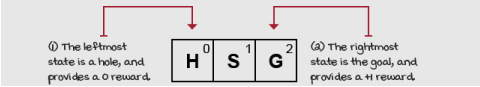
\includegraphics[width=15cm]{images/p000012}
\end{figure}
初始时,Agent位于状态S,左侧状态H为一个洞,是终止状态,获得奖励为0.0;右侧状态G为目标,获得奖励为+1.0,是终止状态。
其MDP环境如下所示:
\begin{figure}[H]
	\caption{Slippery Bandit Walk环境之MDP}
	\label{p000013}
	\centering
	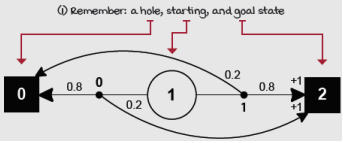
\includegraphics[width=15cm]{images/p000013}
\end{figure}
如上图所示:
\begin{itemize}
    \item Agent在状态S时,选择行动0(向左),进入左侧小黑点:
    \begin{itemize}
        \item 以80\%概率进入状态H,获得奖励0.0并终止;
        \item 以20\%概率进入状态G,获得奖励+1.0并终止;
    \end{itemize}
    \item Agent在状态S时,选择行动1(向右),进入右侧小黑点:
    \begin{itemize}
        \item 以80\%概率进入状态G,获得奖励+1.0并终止;
        \item 以20\%概率进入状态H,获得奖励0.0并终止;
    \end{itemize}
\end{itemize}
但是与第1章不同,我们这里假设我们并不知道这个转移函数。我们要研究在这种情况下,Agent怎样找到最佳策略。
\subsection{贪婪策略}
Agent会首先随机选择一个行动,如果该行动产生正的奖励,之后就一直坚持采用该行动,以SBW环境为例,如图所示:
\begin{figure}[H]
	\caption{SBW环境之Greedy Policy}
	\label{p000014}
	\centering
	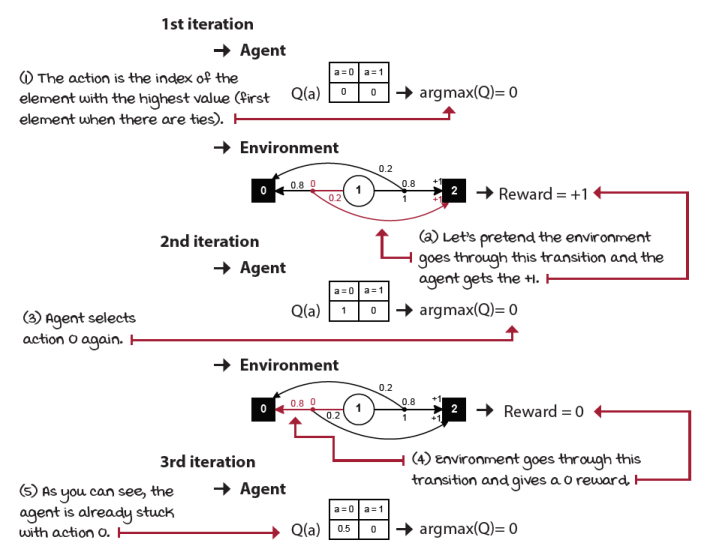
\includegraphics[width=15cm]{images/p000014}
\end{figure}
我们将在状态S能采取的所有行动的Q值设为0,既$\{ 0: 0.0, 1: 0.0 \}$,假设我们初始时在状态S选择行动0(向左),进入左侧实心小点,
此时环境随机进入状态G,因此我们得到了+1.0的奖励,更新Q值为$\{ 0: 1.0, 1: 0.0 \}$,因为我们看到采取行动0可以获得1.0的奖励,因
此我们会一直选择行动0。
当第2次时,我们仍然选择行动0,此时环境随机地转到状态H,此时我们获得的奖励为0.0,我们重新计算Q值:
$q=\frac{1.0 + 0.0}{2}=0.5$,式中分子表示我们分别获得了+1.0和0.0的奖励,分母为我们进行试验的次数。
当第3次时,我们仍然会选择行动0,此时环境随机地转到状态H,我们获得的奖励为0.0,我们重新计算Q值:$q=\frac{1.0 + 0.0 + 0.0}{3}=0.333333$,
分子表示历次试验获得的奖励,分子为试验次数。最终我们策略的Q值为0.2左右。
